\section{Czujnik odległości}
Bardzo popularnym rozwiązaniem problemu omijania przeszkód jest wykorzystanie
czujników ultradźwiękowych. Dane pomiarowe pobrane w pierwszym kroku z sonaru
wykorzystywane są to stworzenia lokalnej reprezentacji otoczenia pozwalającej na
późniejsze sterowanie robotem\cite{ObstaclesAvoidanceIR}. Dla tak zdefiniowanego
problemu możemy wyróżnić dwa rodzaje reprezentacji środowiska. Pierwszy rodzaj
reprezentacji opiera się o siatkę dzięki której środowisko podzielone jest na
skończoną liczbę komórek które mogą posiadać stan świadczący o pustej przestrzeni
lub obecności przeszkody w danej komórce. Drugim sposobem reprezentacji jest
przedstawienie otoczenia za pomocą zbioru właściwości takich jak punkty, linie
oraz płaszczyzny. Wybór sposobu reprezentacji jest z reguły podyktowany
rodzajem problemu jaki stawiany jest przed robotem mobilnym.

Innym rodzajem czujników bardzo dobrze sprawdzających się w rozwiązywaniu
problemu omijania przeszkód są dalmierze oparte o czujnik podczerwieni. Często
zdarza się, iż dalmierze IR\footnote{IR (ang. infrared) - skrótowe oznaczenie
urządzeń wykorzystujących podczerwień do swojego działania} są wybierane ze
względu na ich bardzo krótki czas odpowiedzi w porównaniu do czujników
ultradźwiękowych. Niestety jakość pomiaru w przypadku
czujników podczerwieni jest w dużym stopniu zależna od współczynnika odbicia
powierzchni przeszkody, jak również odległości od przeszkody oraz położenia
nadajnika i odbiornika w~stosunku do powierzchni przeszkody. Zdarza się więc, że
brak precyzyjnych danych o~lokalizacji przeszkody i jej właściwościach
wykluczają dalmierze IR z niektórych zastosowań. Jednakże szeroka dostępność
tego typu urządzeń oraz łatwość ich wykorzystania spowodowała, że są one
najczęściej stosowane w robotach zajmujących się podążaniem za~ścianą czy
omijaniem i liczeniem przeszkód.

\begin{figure}[h!]
 \centering
 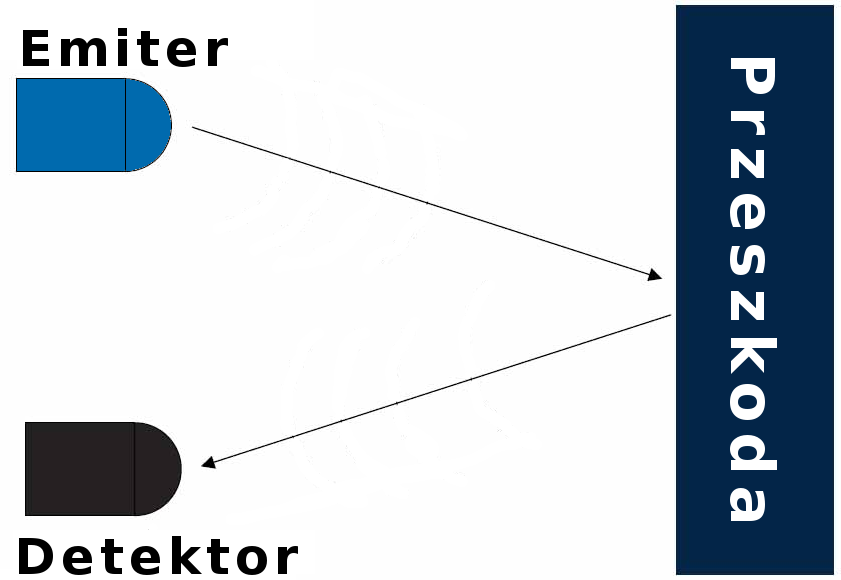
\includegraphics[height=62mm]{../images/ch04/ir_sensor.png}
 \caption{Zasada działania dalmierza wykorzystującego podczerwień}
 \label{fig:IRSensors}
\end{figure}

Typowy dalmierz IR składa się z dwóch elementów. Pierwszym z nich jest dioda
emitująca promieniowanie podczerwone, natomiast drugim elementem jest detektor
najczęściej fotodioda lub fototranzystor. 
Zasada działania tak zbudowanego
czujnika odległości opiera się o zjawisko odbicia. Światło wyemitowane przez
emiter odbija się od przeszkody i trafia do detektora. Niestety pomiar tego
rodzaju jest niezwykle wrażliwy na zmiany w oświetleniu oraz rodzaj i kształt
napotkanej przeszkody.
 
\subsection{Algorytm omijania przeszkód}
Algorytm sterujący ruchami robota bazuje w całości na danych pomiarowych
otrzymanych z czujników robota. Opisane podejście jest adaptacją metodologii
opisanej w ramach pracy ,,Obstacles Avoidance Method for an Autonomous Mobile
Robot'' \cite{ObstaclesAvoidanceIR}. Zaproponowane rozwiązanie bazuje na prostej
maszynie stanów w której przejścia pomiędzy kolejnymi stanami odbywają się
poprzez zmianę poziomów na czujnikach odległości. Autorzy proponują podłączenie
do robota dwóch dalmierzy jednego po lewej (LS), a drugiego po prawej stronie
(RS) robota w taki sposób aby przed robotem nie było martwego punktu. Sposób
montażu czujników został przedstawiony na rysunku poniżej.

\begin{figure}[h!]
 \centering
 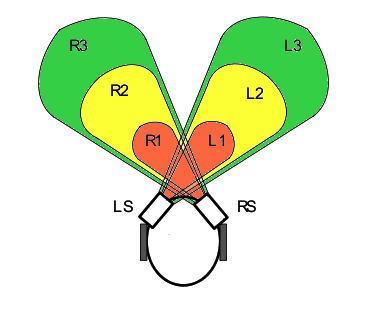
\includegraphics[height=70mm]{../images/ch04/ir_sensor_position.png}
 \caption{Sposób montażu czujników podczerwieni na robocie \cite{ObstaclesAvoidanceIR}}
 \label{fig:IRSensorPosition}
\end{figure}

Każdy z czujników składa się z nadajnika i odbiornika podczerwieni, a ich
przedział czułości, zgodnie z zaleceniami autorów, podzielony został na trzy
poziomy oznaczone symbolami L1, L2, L3 dla czujnika lewego i odpowiednio R1, R2,
R3 dla czujnika prawego. Istotne jest aby kolejne poziomy ułożone były w porządku
rosnącym, a przerwa pomiędzy kolejnymi była na tyle szeroka, aby zminimalizować
wpływ niedokładności pomiaru odległości. W chwili gdy robot znajduje się w ruchu
na każdym z czujników jesteśmy w stanie odczytać wartość odległości od
przeszkody. Dzięki takiej informacji możemy jednoznacznie kontrolować zachowanie
robota w zależności od poziomu jaki w danej chwili ustalił się na poszczególnych
dalmierzach. 

Opierając się na takich założeniach, jeżeli oba czujniki nie
wykrywają na swojej drodze przeszkody to robot porusza się z maksymalną możliwą
prędkością. Gdy jeden z czujników wykryje obecność przeszkody na poziomie  L3
lub/i R3 prędkość poruszania się robota zostanie zmniejszona o połowę. Gdy
przeszkoda znajdzie się w odległości poziomu L2 lub/i R2 prędkość z jaką porusza
się robot zostanie ustalana na 1/4 prędkości maksymalnej. Jeżeli natomiast
przeszkoda zostanie wykryta na poziomie L1 lub/i R1 robot skręci w prawo lub lewo
w zależności od położenia przeszkody i wyznaczonego celu.

Na poniższym rysunku zaprezentowane zostały cztery najbardziej typowe ze
wszystkich z możliwych sytuacji oraz definicja manewru jaki robot
podejmie, aby skutecznie ominąć napotkaną przeszkodę. 

\begin{figure}[h!]
 \centering
 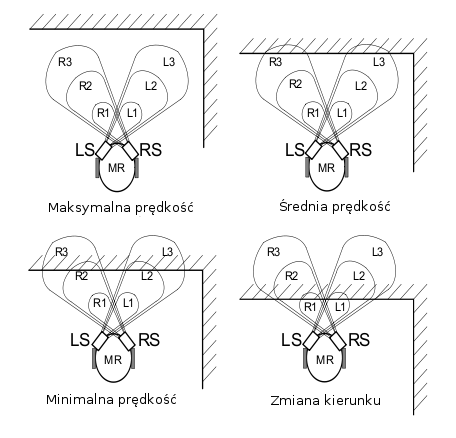
\includegraphics[height=140mm]{../images/ch04/obs_avoid_algorithm.png}
 \caption{Przykładowe sytuacje i definicja reakcji robota}
 \label{fig:IRSensorPosition}
\end{figure}

Uogólniając zasadę działania algorytmu, robot dostosowuje swoją prędkość na
podstawie aktualnej odległości od przeszkody odczytanej z czujników odległości.
W chwili gdy robot znajdzie się bezpośrednio przed przeszkodą skręci on w prawo
lub lewo aby ją ominąć. Kąt o jaki wykonany zostanie zakręt zależy od tego na
którym czujniku przeszkoda została wykryta oraz aktualnego celu do którego robot
zmierza. Szczegółowy opis poszczególnych możliwych sytuacji oraz rodzaj akcji
podejmowanej przez robota jest przedstawiony w tabeli na następnej stronie. 

Podane w tabeli wartości mają charakter orientacyjny i w gdy robot ma
wyznaczony cel do którego zmierza kierunki skrętu mogą w niektórych przypadkach
ulec zmianie. Mogą również pojawić się dodatkowe zmiany kierunku jazdy umożliwiające
powrócenie na ścieżkę do wyznaczonego punktu docelowego.

W pierwszych sześciu kolumnach tabeli prezentowany jest stan ustalony na poszczególnych
poziomach odległości z podziałem na czujnik prawy i lewy. Jedynka w odpowiedniej
kolumnie oznacza obecność przeszkody w danym przedziale odległości, natomiast
zerem oznaczany jest brak przeszkody. W ostatniej kolumnie prezentowana jest
akcja jaką podejmie robot po wykryciu danej konfiguracji stanów.

\begin{table}[hb]
\rowcolors{2}{white}{gray!20}
\centering
\caption{Zachowanie robota w zależności od stanu wykrywanego na czujnikach odległości}
   	\begin{tabular}{ | c | c | c | c | c | c | p{4.75cm} |} \hline
   		R3 & L3 & R2 & L2 & R1 & L1 & Akcja robota \\ \hline
   		0  & 0  & 0  & 0  & 0  & 0  & Maksymalna prędkość\\ \hline
   		0  & 1  & 0  & 0  & 0  & 0  & Średnia prędkość \\ \hline
   		0  & 1  & 0  & 1  & 0  & 0  & Minimalna prędkość \\ \hline
   		0  & 1  & 0  & 1  & 0  & 1  & Skręt w lewo o $45\,^{\circ}$ \\ \hline 
   		1  & 0  & 0  & 0  & 0  & 0  & Średnia prędkość \\ \hline
   		1  & 0  & 1  & 0  & 0  & 0  & Minimalna prędkość \\ \hline
   		1  & 0  & 1  & 0  & 1  & 0  & Skręt w prawo o $45\,^{\circ}$  \\ \hline
   		1  & 1  & 0  & 0  & 0  & 0  & Średnia prędkość \\ \hline
   		1  & 1  & 1  & 0  & 0  & 0  & Minimalna prędkość \\ \hline
   		1  & 1  & 1  & 0  & 1  & 0  & Skręt w prawo o $45\,^{\circ}$ \\ \hline
   		1  & 1  & 0  & 1  & 0  & 0  & Minimalna prędkość \\ \hline
   		1  & 1  & 0  & 1  & 0  & 1  & Skręt w lewo o $45\,^{\circ}$ \\ \hline 
   		1  & 1  & 1  & 1  & 0  & 0  & Minimalna prędkość \\ \hline 
   		1  & 1  & 1  & 1  & 0  & 1  & Skręt w lewo o $45\,^{\circ}$ \\ \hline 
   		1  & 1  & 1  & 1  & 1  & 0  & Skręt w prawo o $45\,^{\circ}$ \\ \hline 
   		1  & 1  & 1  & 1  & 1  & 1  & Skręt w lewo o $90\,^{\circ}$ \\ \hline
   	\end{tabular}
\label{ObstacleAvoidTable}
\end{table}
\newpage
\subsection{Implementacja}
W zrealizowanej w ramach pracy magisterskiej implementacji robot, Dark Explorer,
wyposażony został w dwa dalmierze Sharp GP2D12 o efektywnym zasięgu od 10 do 80
cm. Każdy z~dalmierzy wyposażony jest w nadajnik i odbiornik IR. Czujnik
GP2D12 samodzielnie dokonuje pomiaru odległości i zwraca go w postaci sygnału
analogowego. Dlatego też, robot wykorzystuje konwerter analogowo-cyfrowy do
przetwarzania wyniku pomiaru otrzymanego z czujnika. Wartość napięcia otrzymana
na wyjściu z konwertera jest za pomocą równania, otrzymanego na podstawie
charakterystyki wyjściowej dalmierza, zamieniana na odległość czujnika od
przeszkody. Na zdjęciu poniżej zaznaczone zostały poszczególne elementy składowe
czujnika oraz kolejne wyprowadzenia.

\begin{figure}[hb]
 \centering
 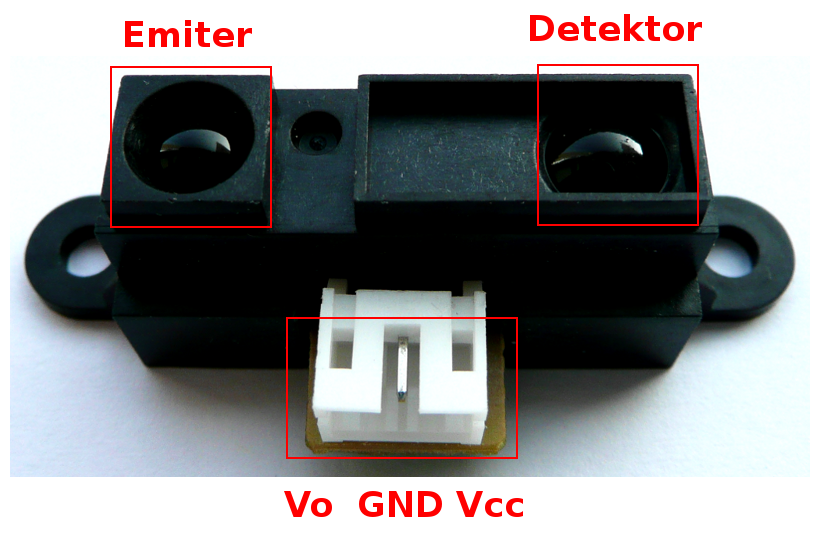
\includegraphics[width=100mm]{../images/ch04/real_gp2d12_view.png}
 \caption{Budowa czujnika GP2D12 wraz z wyporowadzeniami}
 \label{fig:SharpGP2D12}
\end{figure}

Zastosowany czujnik odległości został wyposażony w unowocześniony sposób
dokonywania pomiarów odległości. Użyty dalmierz wykorzystuje triangulację oraz
małą liniową matrycę CCD aby obliczyć odległość od przeszkody w polu
widzenia sensora\cite{website:acroname-robotics}. Podstawową zasadą działania
nowego systemu pomiaru odległości jest wysłanie impulsu światła podczerwonego który po odbiciu od przeszkody wraca
do detektora i tworzy trójkąt pomiędzy emiterem, detektorem a przeszkodą. Kąty w
tym trójkącie zmieniają się razem z odległością od przeszkody, co zostało
zaprezentowane na rysunku \ref{fig:SharpGP2D12_opertaion_theory}.

Kluczem do poprawnego działania takiego rozwiązania jest soczewka która dba o to, aby
odbite światło trafiało na odpowiednie pole matrycy CCD w zależności od wartości
kątów w opisanym powyżej trójkącie. Dzięki takiej budowie soczewki, czujnik na
podstawie danych z matrycy CCD może określić kąt pod jakim światło odbite
wróciło, a dzięki temu jest w stanie obliczyć aktualną odległość od przeszkody.
Zastosowana w dalmierzu metoda pomiaru odległości jest niemal całkowicie odporna
na zakłócenia spowodowane światłem zewnętrznym. Dodatkowo eliminuje błędy
pomiarowe związane z kolorem powierzchni przeszkody. Dzięki zastosowaniu takiego
podejścia możliwe jest wykrycie całkowicie czarnej ściany w całości oświetlonej
przez intensywne światło słoneczne, co w przypadku starszych dalmierzy
praktycznie nie jest możliwe.

\begin{figure}[h!]
 \centering
 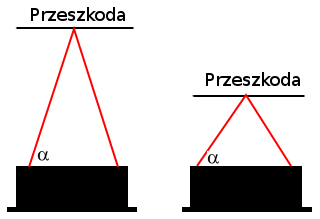
\includegraphics[width=100mm]{../images/ch04/gp2d12_operation_theory.png}
 \caption{Zasada przeprowadzania pomiaru przez czujnik GP2D12}
 \label{fig:SharpGP2D12_opertaion_theory}
\end{figure} 

Zgodnie z założeniami algorytmu obszar zasięgu czujników został podzielony na
trzy poziomy. Poziom trzeci zostały wyznaczony w odległości 50 cm, drugi poziom
wyznaczony został w odległości 25 cm, a poziom pierwszy wyznaczony został w
odległości 12 cm od przeszkody. Program zarządzający działaniem robota odczytuje
kolejno dane o odległości otrzymane z czujnika prawego i lewego i kontroluje
zachowanie robota zgodnie z zasadami przedstawionymi w tabeli
\ref{ObstacleAvoidTable}. Z praktycznego punktu widzenia implementacja tego
rodzaju algorytmu sprowadza się do stworzenia tablicy w której przechowywane są
prędkości poruszania się każdego z czterech kół z uwzględnieniem lokalizacji
czujnika oraz progu odległości w jakim znajduje się przeszkoda.

Aby móc praktycznie wykorzystać dane analogowe uzyskane z dalmierza wykorzystany
został wbudowany w robota przetwornik analogowo-cyfrowy (ADC). Sposób obsługi
przetwornika analogowo-cyfrowego, na potrzeby omijania przeszkód, został
zrealizowany w oparciu o dokumentację i przykłady zawarte w książce J. Augustyna
pt. ,,Projektowanie systemów wbudowanych na przykładzie rodziny SAM7S z rdzeniem
ARM7TDMI''. Zgodnie ze specyfikacją, przetwornik, wbudowany w procesor SAM7S
pozwala na przetwarzanie napięcia w granicach od 0V do napięcia referencyjnego
które w przypadku robota Dark Explorer jest równe napięciu zasilania procesora
tj. 3.3V. Aby uzyskać jak najdokładniejszy wynik pomiaru
przetwornik został skonfigurowany do pracy z rozdzielczością 10-bitową. Wydłuża to czas potrzebny na
konwersję danych jednakże przy prędkościach z jakimi robot się porusza nie ma to
większego wpływu na jakość działania aplikacji gdyż wykorzystany przetwornik
ADC mierzy i zwraca wartość chwilową napięcia\cite{JAugustyn}.

W trakcie działania aplikacji uruchamiany jest proces konwersji na kanałach do
których podłączone są czujniki odległości, a następnie aplikacja oczekuje na
wywołanie przerwania związanego z wpisaniem wartości na temat napięcia do
odpowiednich rejestrów. Po otrzymaniu wartości napięcia widocznego na wyjściu z
dalmierzy, obliczana jest odległość w jakiej znajduje się przeszkoda. Ze względu
na zastosowaną metodę pomiarową napięcie wyjściowe z czujników odległości nie ma
charakterystyki liniowej. Jest to związane obliczeniami trygonometrycznymi
wykonywanymi w celu wyznaczenia odległości od przeszkody. 
W tym celu,
udostępniona w ramach dokumentacji czujnika\cite{GP2D12DataSheet} charakterystyka
wyjściowa, posłużyła do wyznaczenia progów napięcia dla zdefiniowanych przez
algorytm progów odległości.
% W tym celu,
% udostępniona w ramach dokumentacji czujnika\cite{GP2D12DataSheet} charakterystyka
% wyjściowa, posłużyła do wyznaczenia równania pozwalającego z zadowalającą
% dokładnością wyznaczyć odległość od przeszkody. 
% W wyniku dopasowania otrzymano
% równanie postaci.
% \begin{equation}
% y=\frac{a+bx}{1+cx+dx^2}
% \end{equation}
% Powyższe równanie nie odzwierciedla w pełni charakterystyki czujnika, ale w
% bardzo dobry sposób przybliża ją w przedziale wymaganym do prawidłowej
% implementacji algorytmu. Posiadając tak przygotowane dane zaimplementowanie
% reszty algorytmu nie stanowiło już większej trudności. 

W ramach testów przeprowadzono kilka symulacji działania implementacji dla
różnych pozycji startowych przy zbliżaniu się robota to brzegu przeszkody. Już
pierwsze testy wykazały, że gdy robot porusza się prostopadle do płaszczyzny
ściany algorytm działa bardzo dobrze, jednakże w przypadku gdy ruch ten nie jest
prostopadły w niektórych przypadkach pojawiają się problemy z działaniem
algorytmu. Wspomniane problemy związane są z w niektórych przypadkach z
odbieraniem przez dalmierz dodatkowych sygnałów wysłanych z sąsiedniego czujnika.
Rozwiązaniem takiego problemu mogłoby być zastosowanie czujników z kodowaniem
sygnału. Co więcej zasada działania dalmierzy IR nie pozwala na wykrycie małych i
wąskich obiektów stawianych na drodze robota. Dodatkowym problemem jest
nieliniowość charakterystyki czujnika która przy odległości mniejszej od 10cm
wskazuje napięcia które mogą być mylnie zinterpretowane.
